\begin{figure*}[t]
\centering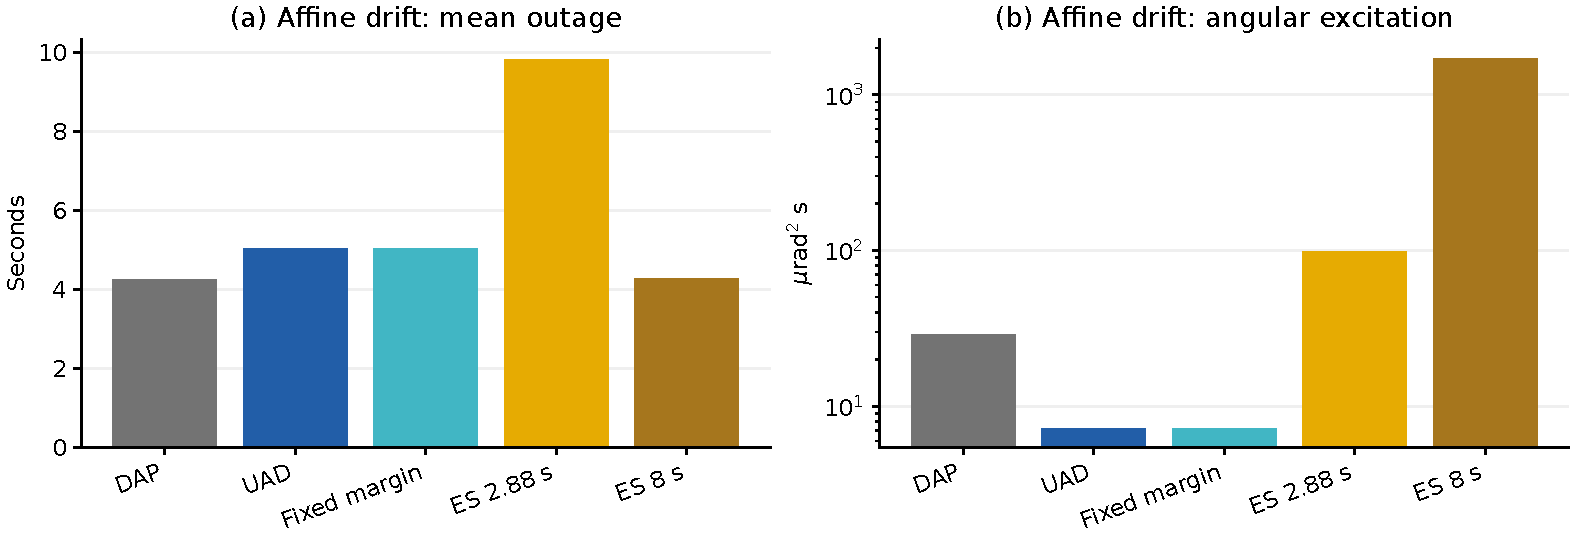
\includegraphics[width=\textwidth]{budget_tradeoff.pdf}
\caption{New paired affine-drift results. The native eight-second tracker has substantially more angular excitation than the time-matched tracker. Fixed-margin and UAD trajectories coincide in every tested pair. No tracker receives fault-diagnosis credit.}
\label{fig:budget}
\end{figure*}

\section{Separate Verification and Controlled Comparisons}
\subsection{Proof and measurement-event audit}
A separate Python implementation, without importing the MATLAB simulator, truth generator, evaluator, or reporting code, maximizes the angular expression by eliminating $e_0$ analytically and optimizing the direction of $d$ on its boundary. Across 1,200 cases, including zero radii, zero increments, noncentered balls and negative angular loss, no excess exceeds floating-point tolerance. The largest centered sharpness difference is $4.55\times10^{-13}$ $\mu$rad$^2$. A further 9,600 direct optical-ratio tests verify the power conversion and radian--microradian scaling. These calculations corroborate the analytic proof; they are not an independent human or formally rounded proof.

For the measurement event, $\Pr(|Z|>\kappa)=\delta/(5N)$ follows from the two-sided Gaussian tail. Thus $\Pr(\mathcal E^c)\leq\sum_{i,j}\Pr(|Z_{ij}|>\kappa)=\delta$. For any observation-selected index $\tau$, on $\mathcal E$ the interval contains $p_\tau$; hence $\{\overline p_\tau<p_{\min},p_\tau\geq p_{\min}\}\subseteq\mathcal E^c$. This establishes the stated false-enablement bound without optional-stopping independence. It does not establish fit coverage or protect against a future fault jump.

On $\mathcal E$, $\eta<1$ makes $1+\sigma_pZ_p>0$, so the zero clamp is inactive whenever true power is positive. At true zero power, both measured power and interval endpoints are zero. If $\eta\geq1$, the implementation retains an unbounded upper endpoint and cannot enable acquisition from that interval. Non-Gaussian or biased errors do not inherit this calibration.

In 10,000 independent synthetic missions with 700 samples and five channels, the complete envelope fails in 100 missions. An intentionally adverse minimum-measurement selection produces eight false acquisition enablements, all outside the event; pointwise 99\% intervals at that selected time produce 9,680. With variance-normalized Student-$t_5$ disturbances, the same Gaussian envelope fails in 997/1,000 separate missions and adverse-time acquisition is false in 477/1,000. Equal variance therefore does not justify transferring the calibration to heavy tails. These are illustrative selection stress tests, not the plant's trigger. The separate raw-trace audit also reconstructs the exact three-consecutive-residual adaptive trigger used by the plant algorithm.

\subsection{Actuator and raw-record verification}
Independent Python RK4 slope recurrences agree with all six exported discrete maps to $1.78\times10^{-15}$ maximum entry error. Independently reconstructed finite impulse and stage bounds agree with all eight candidate tubes to $2.29\times10^{-20}$ rad and reproduce 33,024 stage constraint checks. This verifies the finite construction numerically. Neither endpoint checks nor successful intermediate simulations prove enclosure for a continuous parameter rectangle.

The Python audit reads all 29,250 V4 traces, reconstructs optical power, trigger, delivered increment, power lower bound, premise flags, violations, outage, excitation, acceptance and coverage, and checks every entry of the 36-row primary table. Across primary and sensitivity conditions, 2,121 UAD probes have a calculated bound; 1,564 satisfy checked premises, with zero observed bound violations. The remaining 557 include all 100 sensitivity bound violations. These heterogeneous selected counts do not define a homogeneous field-failure population.

Original V4 traces did not store the offset history or every standardized noise channel. The checker independently reimplements the documented injection formula and uses the saved maximum-noise scalar for the missing rate-channel history; it does not call the MATLAB generator. The new revision logs complete offset and noise histories, which are checked directly. This distinction prevents overstating independence or claiming missing historical measurements were available.



\subsection{Fixed-margin and time-matched comparison}
The new protocol freezes source/configuration before 7,200 comparisons and 3,000 actuator-grid trials. New seeds 5001--5050 evaluate all nine scenarios under nominal sensing, fivefold noise, $[2,-1]\um$ bias, and $0.9\alpha$ early-trigger conditions. All methods share the trigger. UAD, the fixed-margin selector and ES have a 2.88-s diagnostic-excitation time cap; their candidate dwells are 0.36~s. Historical DAP retains its original 0.35/0.50-s library; every selected DAP probe in these records lasts 2.8~s. This exception to the frozen descriptor is disclosed without changing outcomes. This is a time-matched comparison; realized angular energy and reference amplitude need not match.

The simpler selector retains the same sensor gate, optical-relative bound, candidate rank checks and precomputed constraint validity, but replaces the model-dependent delivered-motion radius by a fixed $2\um$ guard plus the current encoder envelope. The guard is declared before outcomes and is a robustness heuristic, not a proven enclosure. It isolates the practical value of the finite-model radius without inventing a new guaranteed baseline. A logged model-premise flag does not make this heuristic a certified UAD probe.

A separate native ES extension uses the identical seeds and conditions with eight seconds of excitation, adding 1,800 runs. It is declared before its own outcomes, after the matched evaluation; no parameter is selected from either set. This provides paired native/time-matched evidence rather than comparing different seed populations. ES remains a tracker and receives no fault-diagnosis acceptance credit.

\begin{table*}[t]
\caption{New revision comparisons: 50 paired seeds per row. All methods except native ES share a 2.88-s excitation-time cap. The fixed margin is heuristic. Energy is angular excitation. BV counts all observed lower-bound failures, including out-of-model runs; zero is not a reliability claim. Complete acceptance, rejection, false correction and confidence-miss counts are supplied.}
\centering\footnotesize
\begin{tabular}{llrrrrr}\toprule
Condition/scenario & Method & Accepted & Outage (s) & Energy ($\mu$rad$^2$s) & False acquisition & BV\\\midrule
\ReviewRows
\bottomrule\end{tabular}
\label{tab:review}
\end{table*}

At nominal affine drift, mean outage is \NewUADDrift~s for UAD, \NewDAPDrift~s for DAP, and \NewGuardDrift~s for the fixed margin. Time-matched ES reaches \NewESDrift~s, versus \NewNativeDrift~s in its native mode. Table~\ref{tab:review} retains the corresponding diagnosis counts and energy. The fixed-margin and UAD selectors produce exactly identical power, angle and probe trajectories in all 2,800 paired comparison/grid cases. The experiments therefore demonstrate no practical outcome advantage for the more elaborate tube over this heuristic on the tested conditions. Its distinction is a conditional finite-model justification, not superior observed recovery. These are costs and tradeoffs; they are not evidence that a certificate generally improves recovery.

The actuator stress test crosses five inertias $J_a/J_0\in\{.8,.91,1,1.13,1.25\}$ with five lags $\tau_a/\tau_0\in\{1,1.12,1.25,1.37,1.5\}$, for two scenarios, three methods and 20 new seeds per point. Interior values are deliberately outside the finite-model theorem. Per-point outcomes and observed tube failures are retained; success at these points does not close the continuous-interval gap.

All 12,000 new traces are checked by the separate Python implementation, including recorded offsets and all noise channels. Reports distinguish valid-model flags, rejected premises, bound failures, acceptance, rejection, missed diagnoses, false corrections, offsets accepted with error above $1\um$, and confidence misses. Paired outage contrasts use 5,000 whole-seed bootstrap draws; descriptive 95\% and approximate family-36 limits are supplied for each comparator's condition/scenario family. Planner runtime is recorded on MATLAB R2026a, Apple silicon; it excludes offline library generation and is not an embedded worst-case guarantee.
